
\documentclass[conference,onecolumn]{IEEEtran}
\usepackage[encapsulated]{CJK}
\usepackage{cite}
\usepackage{amsmath,amssymb,amsfonts}
\usepackage{algorithmic}
\usepackage{graphicx}
\usepackage{tikz}
\usetikzlibrary{arrows,decorations.pathreplacing,calc}
\usepackage{tabularx}
\usepackage{booktabs}
\usepackage{color}

\begin{document}
\begin{CJK}{UTF8}{bsmi}
\section*{Extracted Content}

\begin{table}[htbp]
\caption{nFAPI Delay Management Timing Offset Parameters~\cite{nfapi_spec}}
\label{tab:delay_mgmt_offsets}
\begin{center}
\begin{tabularx}{\columnwidth}{X|X}
\toprule
\textbf{Parameter} & \textbf{Description} \\ \midrule
Timing offsets (DL\_TTI, UL\_TTI, UL\_DCI, Tx\_Data) & The timing offset ($\mu$s) before the slot start that the corresponding request must be received at PHY. \\ \bottomrule
\end{tabularx}
\end{center}
\end{table}

\hrulefill\par\vspace{1cm}

\begin{table}[htbp]
\caption{nFAPI Timing Info Parameters~\cite{nfapi_spec}}
\label{tab:timing_info}
\begin{center}
\begin{tabularx}{\columnwidth}{l|X}
\toprule
\textbf{Field} & \textbf{Description} \\ \midrule
\textbf{Last SFN / Slot} & Triggering SFN/Slot. \\ 
Time Since Last Info & Time since last report (ms). \\ 
Jitter & DL\_TTI, TX\_DATA, UL\_TTI, UL\_DCI. \\ 
Latest Delay & DL\_TTI, TX\_DATA, UL\_TTI, UL\_DCI from the latest time acceptable ($\mu$s). \\ 
Earliest Arrival & DL\_TTI, TX\_DATA, UL\_TTI, UL\_DCI from the latest time acceptable ($\mu$s). \\ 
Subcarrier Spacing & SCS index (TS38.211). \\ \bottomrule
\end{tabularx}
\end{center}
\end{table}

\hrulefill\par\vspace{1cm}

\begin{table}[htbp]
\caption{nFAPI Delay Management Configuration Parameters}
\label{tab:delay_mgmt_config}
\begin{center}
\begin{tabularx}{\columnwidth}{l|X}
\toprule
\textbf{Parameter} & \textbf{Description} \\ \midrule
timingWindow & Duration of the sliding window used for delay calculation. \\
timingMode & Reporting mode for Timing Info: Periodic, Aperiodic, or Both. \\
timingPeriod & Transmission interval for Timing Info messages. \\ \bottomrule
\end{tabularx}
\end{center}
\end{table}

\hrulefill\par\vspace{1cm}

\begin{figure}[htbp]
  \centerline{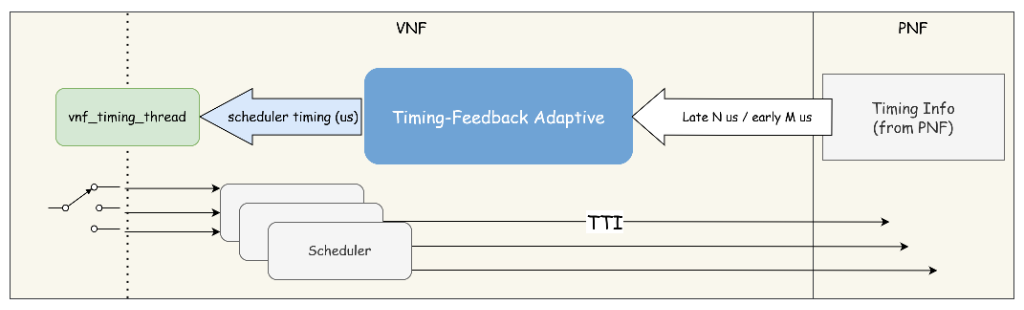
\includegraphics[width=1\columnwidth]{figures/system_model.png}}
  \caption{System Model of the Timing-Feedback Adaptive Scheduler.}
  \label{fig:system_model}
\end{figure}

\hrulefill\par\vspace{1cm}

\begin{equation}
    \Delta t_{offset} = \frac{(t_2 - t_1) - (t_4 - t_3)}{2}
\end{equation}

\hrulefill\par\vspace{1cm}

\begin{equation}
    T_{owd} = \frac{(t_4 - t_1) - (t_3 - t_2)}{2}
\end{equation}

\hrulefill\par\vspace{1cm}

\begin{equation}
    \Delta t_{total} = \Delta t_{offset} + T_{margin}
\end{equation}

\hrulefill\par\vspace{1cm}

\begin{equation}
    N_{slot} = \lfloor \frac{\Delta t_{total}}{T_{slot}} \rfloor
\end{equation}

\hrulefill\par\vspace{1cm}

\begin{equation}
    T_{us} = \Delta t_{total} \pmod{T_{slot}}
\end{equation}

\hrulefill\par\vspace{1cm}

\begin{equation}
    A_{us} = -T_{us}
\end{equation}

\hrulefill\par\vspace{1cm}

\begin{equation}
    A_{slot} = N_{slot}
\end{equation}

\hrulefill\par\vspace{1cm}

\begin{equation}
    N_{skip} = \lfloor \frac{\Delta t_{accumulated}}{T_{slot}} \rfloor
\end{equation}

\hrulefill\par\vspace{1cm}

\begin{figure}[htbp]
  \centerline{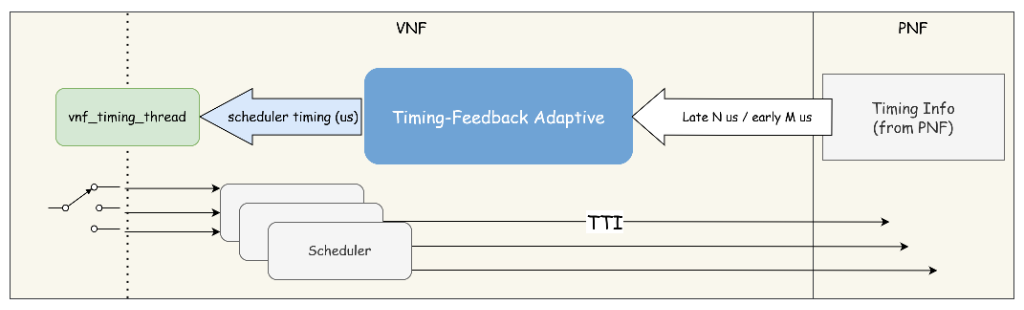
\includegraphics[width=1\columnwidth]{figures/receiving_window.png}} % Placeholder for Figure 2-11
  \caption{Receiving Window mechanism at the PHY}
  \label{fig:receiving_window}
\end{figure}

\hrulefill\par\vspace{1cm}

\begin{figure}[htbp]
\centering
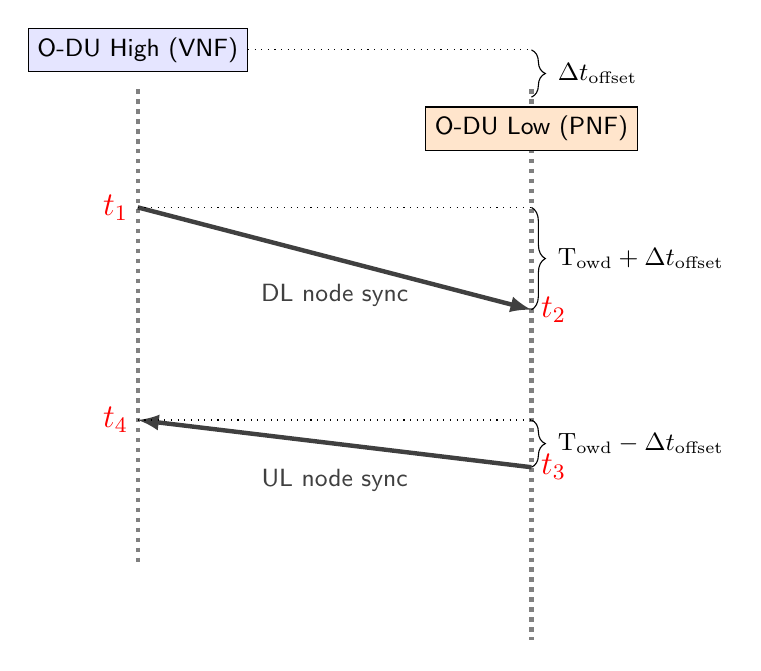
\begin{tikzpicture}[>=latex, font=\small]

% Use sans-serif for node labels to match style
\tikzstyle{block} = [draw, fill=blue!10, rectangle, minimum height=1.5em, minimum width=6em, align=center]
\tikzstyle{block2} = [draw, fill=orange!20, rectangle, minimum height=1.5em, minimum width=6em, align=center]

% Vertical Lines (Timelines)
\draw[dotted, ultra thick, color=gray] (0, 0) -- (0, -6);
\draw[dotted, ultra thick, color=gray] (5, 0) -- (5, -7);

% Top Nodes
\node[block, fill=blue!10] (VNF) at (0, 0.5) {\textsf{O-DU High (VNF)}};
\node[block2, fill=orange!20] (PNF) at (5, -0.5) {\textsf{O-DU Low (PNF)}};

% Offset braces at top
\draw[dotted] (VNF.east) -- (5, 0.5);
\draw[decorate, decoration={brace, amplitude=5pt}] (5, 0.5) -- (5, -0.1) node[midway, right=6pt] {$\Delta t_{\text{offset}}$};

% T1 -> T2 (DL Node Sync)
\coordinate (t1) at (0, -1.5);
\coordinate (t2) at (5, -2.8);
\draw[->, ultra thick, darkgray] (t1) -- (t2) node[midway, below=5pt] {\textsf{DL node sync}};
\node[left, red, font=\large] at (t1) {$t_1$};
\node[right, red, font=\large] at (t2) {$t_2$};

% T1/T2 braces
\draw[dotted] (t1) -- (5, -1.5);
\draw[decorate, decoration={brace, amplitude=5pt}] (5, -1.5) -- (5, -2.8) node[midway, right=6pt] {$\text{T}_{\text{owd}} + \Delta t_{\text{offset}}$};


% T3 -> T4 (UL Node Sync)
\coordinate (t3) at (5, -4.8);
\coordinate (t4) at (0, -4.2);
\draw[->, ultra thick, darkgray] (t3) -- (t4) node[midway, below=5pt] {\textsf{UL node sync}};
\node[right, red, font=\large] at (t3) {$t_3$};
\node[left, red, font=\large] at (t4) {$t_4$};


% T3/T4 braces
\draw[dotted] (t4) -- (5, -4.2);
\draw[decorate, decoration={brace, amplitude=5pt}] (5, -4.2) -- (5, -4.8) node[midway, right=6pt] {$\text{T}_{\text{owd}} - \Delta t_{\text{offset}}$};

\end{tikzpicture}
\caption{Delay Management Procedure (Node Sync)}
\label{fig:latency_probe}
\end{figure}

\hrulefill\par\vspace{1cm}

\begin{table}[htbp]
\caption{DL Node Sync parameters}
\label{tab:dl_node_sync}
\begin{center}
\begin{tabularx}{\columnwidth}{l|X}
\toprule
\textbf{Field} & \textbf{Description} \\ \midrule
t1 & Offset from VNF SFN/slot 0/0 (0..10239999 $\mu$s). \\ \midrule
Delta SFN/slot & Slot shift update (-163839..163839). Negative pulls timeline. \\ \midrule
Sub-carrier spacing & SCS index (0: 15kHz .. 4: 240kHz). \\ \bottomrule
\end{tabularx}
\end{center}
\end{table}

\hrulefill\par\vspace{1cm}

\begin{table}[htbp]
\caption{UL Node Sync parameters}
\label{tab:ul_node_sync}
\begin{center}
\begin{tabularx}{\columnwidth}{l|X}
\toprule
\textbf{Field} & \textbf{Description} \\ \midrule
t1 & The supplied t1 field from DL Node Sync (0..10239999 $\mu$s). \\ \midrule
t2 & Reception time of DL Node Sync at PNF (0..10239999 $\mu$s). \\ \midrule
t3 & Transmission time of UL Node Sync at PNF (0..10239999 $\mu$s). \\ \bottomrule
\end{tabularx}
\end{center}
\end{table}

\hrulefill\par\vspace{1cm}


\bibliographystyle{IEEEtran}
\bibliography{references}
\end{CJK}
\end{document}
